\chapter{Method}

The question to be researched is whether an adaptive bucket-table can be made to do ranking more efficient than a static table with offline updates.

\section{Problem description revisited}

The Companys current ranking algorithm is an implementation of the algorithm Bucket with Global Query. The highscores are stored in Google App Engines Datastore as entities with properties username and a score. A background job  periodically iterates through the highscores making the bucket-table that contains ranks and scores needed to make the estimates. The entities are indexed on highscore-property which is essential to make the process of iterating through the whole set doable.

An exerpt from the bucket-table may look like table \ref{table:ranking-table}. For example, to estimate rank for score $2\;050$ which falls in bucket 6, start by calculating what the score range in bucket 6 is, in this case $2\;204 - 1\;961 = 243$. $2\;050$ is $89$ scorepoints in the bucket and hence the rank is calculated as $83 + 23 \times \frac{89}{243} \approx 91$. See figure \ref{fig:interpolation} for a visual representation of the example.


\begin{table}[h]
  \begin{center}
  \begin{tabular}{ c c c c }
  Bucket no & Start score & Start rank & Size \\
  5 & 1 515 & 83 & 22 \\ 
  6 & 1 961 & 105 & 23 \\ 
  7 & 2 204 & 128 & 23 \\ 
  8 & 2 574 & 151 & 24 \\  
  9 & 2 852 & 175 & 25 \\ 
\end{tabular}
\caption{Excerpt from bucket-table}
\label{table:ranking-table}
\end{center}
\end{table}

\begin{figure}[h!]
  \centering
  \caption{Linear interpolation of rank for score 2050}
  \label{fig:interpolation}
  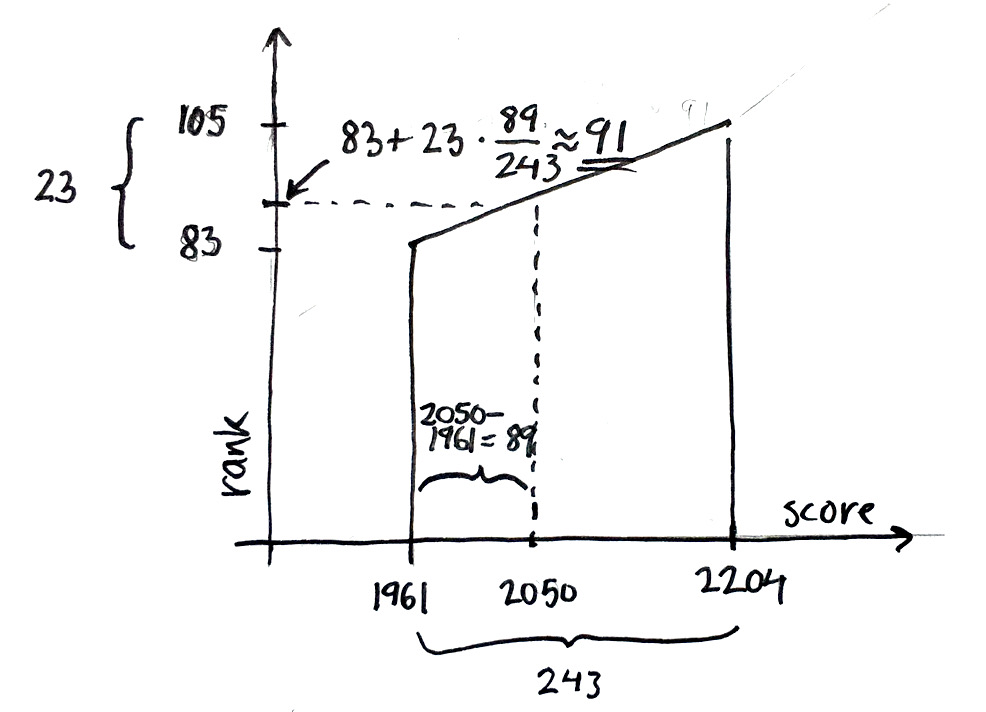
\includegraphics[width=8cm]{img/interpolation.jpg}
\end{figure}

\section{Hypothesis} 

\begin{figure}[h]
  \centering
  \caption{Error over time}
  \label{fig:errortime}
  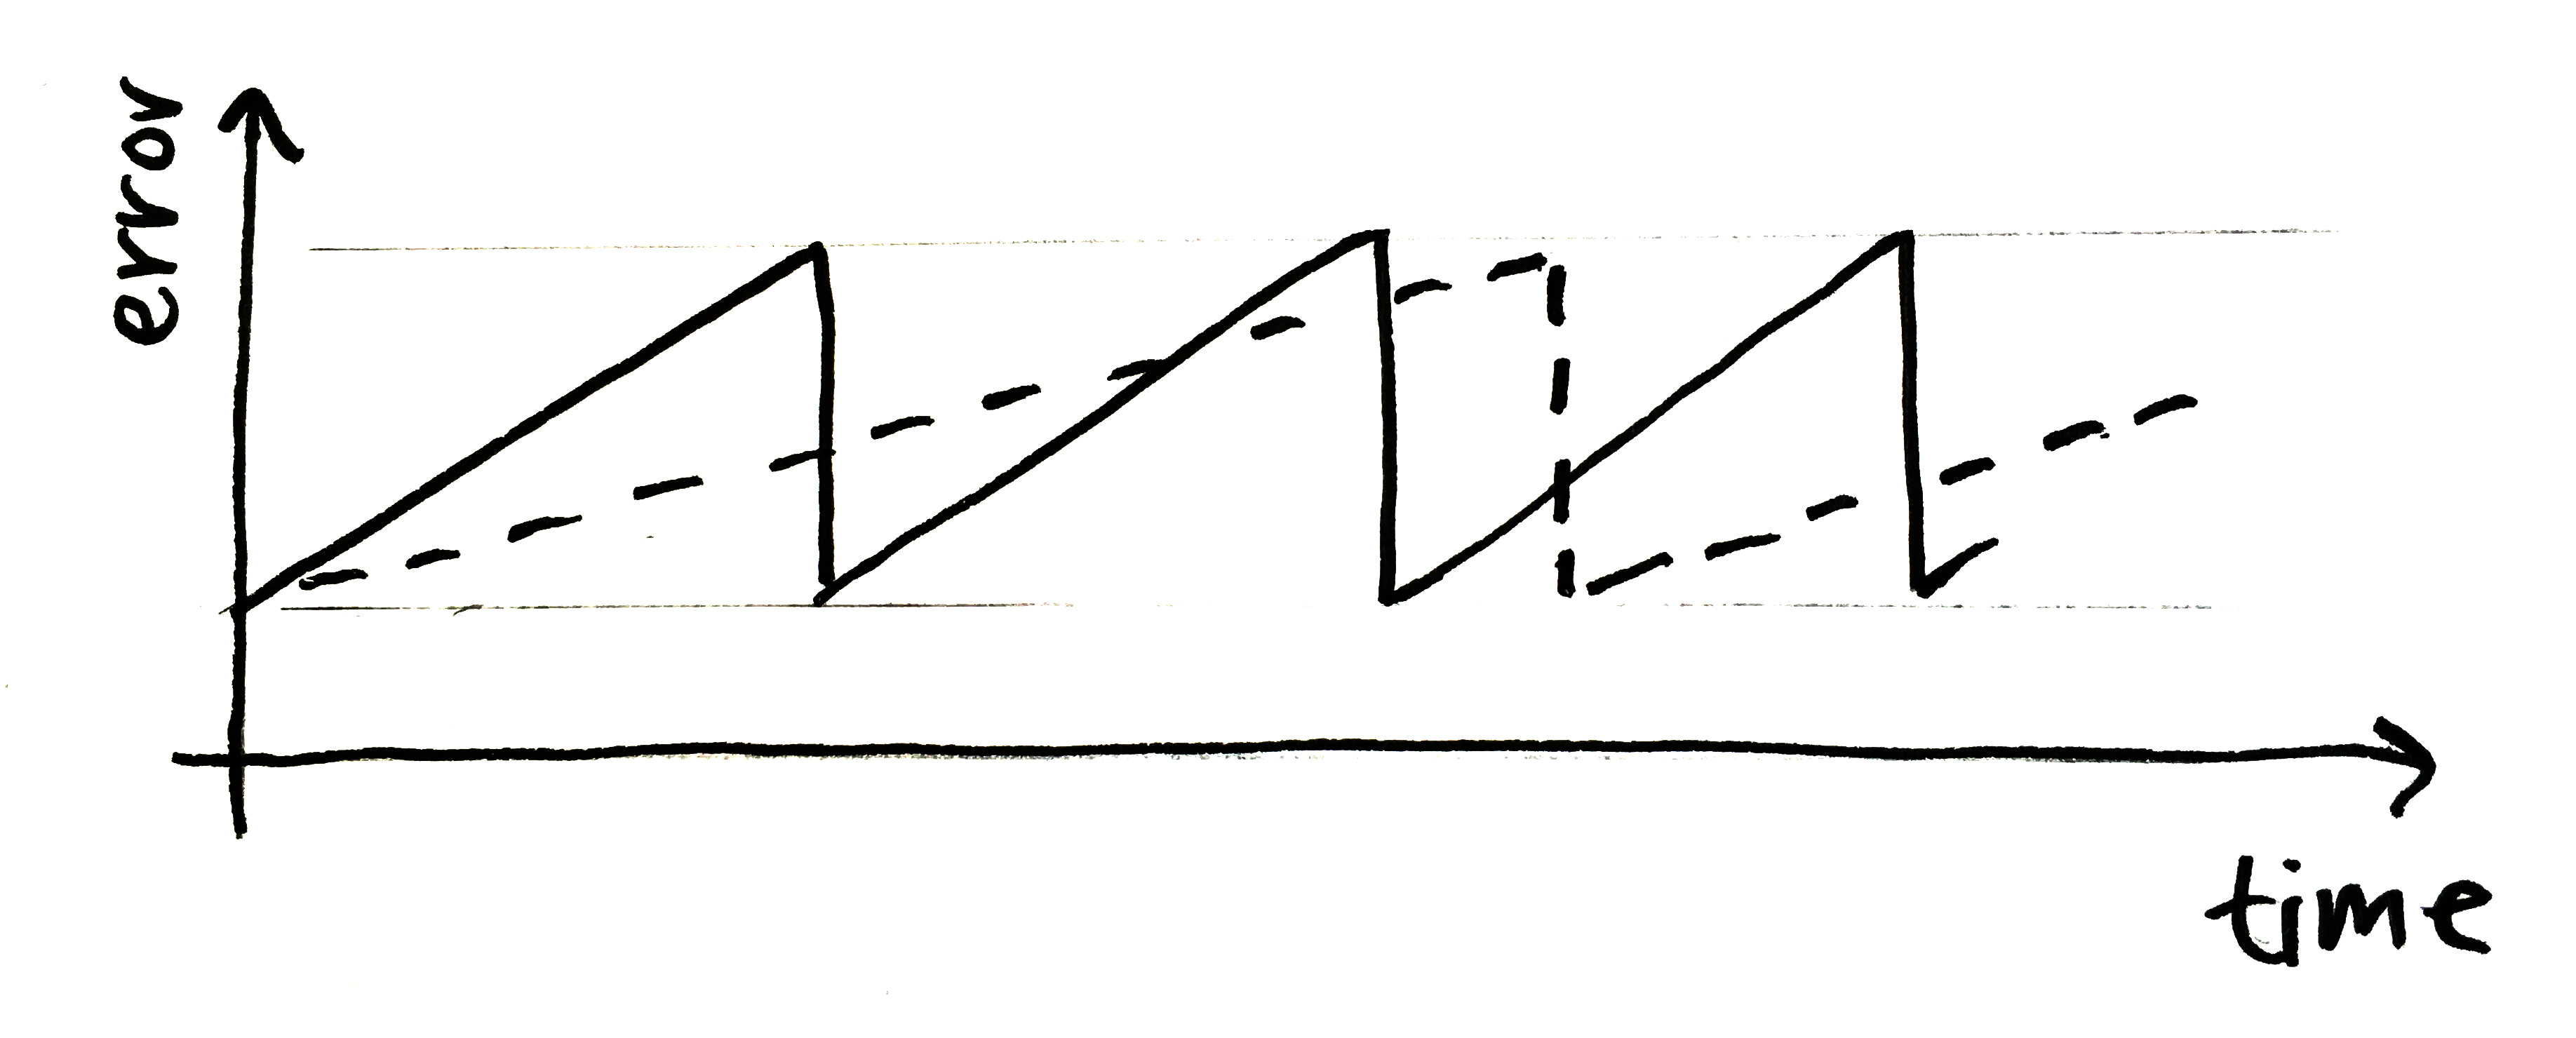
\includegraphics[width=8cm]{img/hypothesis2.jpg}
\end{figure}

\begin{figure}[h]
  \centering
  \caption{Error over time}
  \label{fig:errortime}
  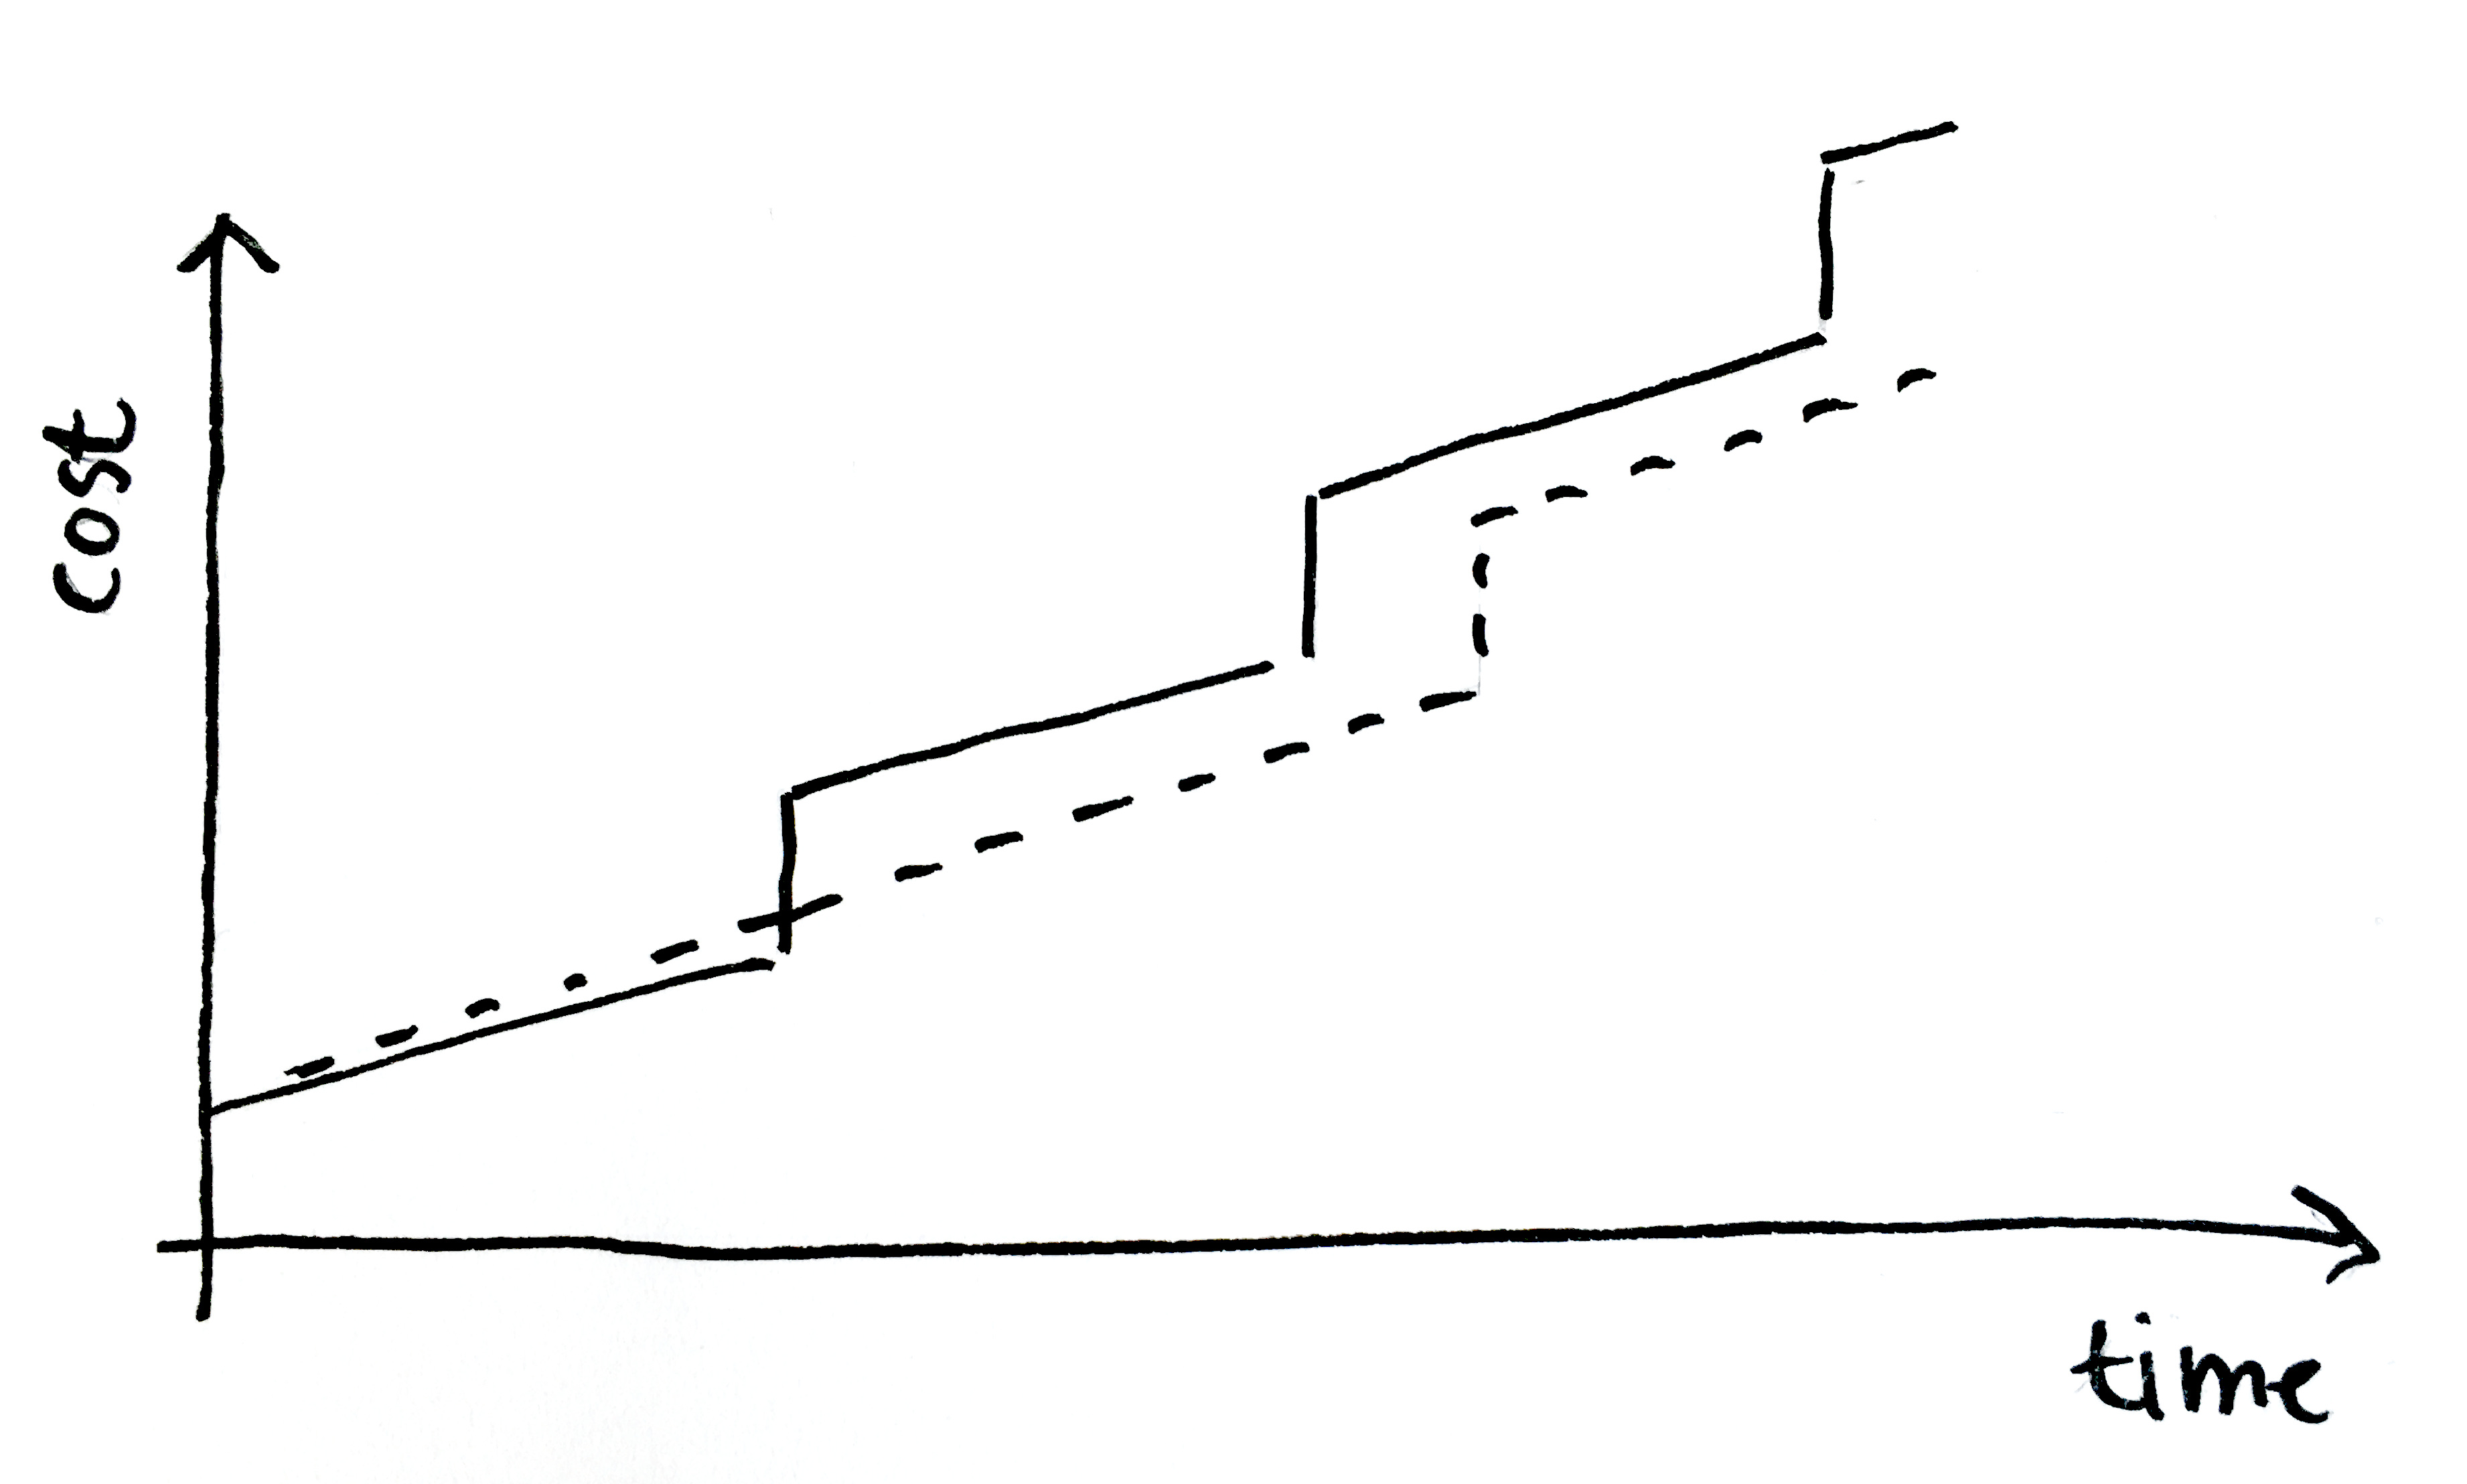
\includegraphics[width=8cm]{img/hypothesis.jpg}
\end{figure}



\section{Data}

The reason for using synthetic data is mainly practical. The production system cannot be altered in such a way that real world data could be tapped within this experiments timeframe. Also, an experiment with real world data would either take a full week to conduct or have to make serveral assumptions rendering the experiment no more authentic than the one with syntetic data that will be used.

On the flip-side, the distribution of the scores is well known. 2) synthetic input to the experiment may be of a more generic nature than real world data. 3) The different characteristics of data in the start and the end of the experiment are not too interesting even from a practical point of view since they only represent a minor part of the total workload.

\begin{shaded}

  Distribution of highscores?

  Distribution over time?
 
\end{shaded}

\section{What and how to measure}

\begin{shaded}
  Measure relative error and execution time

  Number of datastore accesses

  Total execution time (update score + ranking)
\end{shaded}





\section{Limitations}

The data set grows over time. Will be ignored, only focus on case when the set of highscores are reasonably large.

